\documentclass{article}
\usepackage[utf8]{inputenc}
\usepackage{graphicx}

\title{Esperienza di Frank-Hertz}
\author{Francesco Pio Merafina, Onofrio Davide Caputo, Alessandro Lamesta}
\date{}

\begin{document}

\maketitle
\section{Abstract:}
L’esperimento replicato in laboratorio è l'esperimento di Franck-Hertz i quale è una dimostrazione dell’esistenza di livelli energetici stazionari discreti negli atomi
~
\section{Cenni teorici:}
L'idea teorica alla base dell'esperimento è quella che, osservando i tipi di urti degli elettroni con atomi di Ne o Hg entrambi allo stato gassoso, si può osservare se effettivamente gli atomi hanno dei livelli energetici discreti dove alloggiano gli elettroni. Se l'urto elettrone-atomo è di tipo elastico allora l'elettrone ha energia diversa da un generico multiplo intero del gap energetico stato ground e primo stato eccitato, e raggiungerà l'anodo; se l'urto è anelastico l'elettrone ha energia pari ad un generico multiplo intero del gap energetico e quindi non riuscirà a raggiungere l'anodo. Osservando la corrente sull'anodo e come essa vari in funzione della tensione acceleratrice possiamo osservare il valore di questi gap energetici.
~
\section{Apparato sperimentale:}
Per eseguire questo esperimento si è utilizzato un apparato, che consiste in:
\begin{itemize}
    \item Tubo contenente gas Ne oppure Hg riscaldato a 165°C
    \item catodo riscaldato che emette elettroni per effetto termoionico
    \item 3 generatori, uno fisso per regolare il flusso di elettroni U\ped{1}, uno variabile per cambiare l'energia cinetica degli elettroni U$_{2}$, ed uno fisso che serve per selezionare gli elettroni che arrivano all'anodo U$_{3}$
    \item computer con programma CASSY che analizza la differenza di potenziale nell'anodo in cui scorre la corrente degli elettroni che arrivano
\end{itemize}
~
\section{Metodologia di misura:}
Il primo gas usato è stato Ne, più facile da usare poichè non va riscaldato, si è collegato il tubo all'apparato sperimentale e si sono fissati i valori di U$_{1}$ e di U$_{3}$, si è fatto variare il valore di U$_{2}$ ed il programma ha raccolto i dati e restituito un primo plot grezzo dei dati; questa procedura è stata ripetuta a diversi valori di U$_{1}$ e di U$_{3}$. Per Hg si è dovuto prima far evaporare il mercurio portandolo a 165°C poichè a temperatura ambiente il mercurio si trova allo stato liquido, e poi si è proceduto in maniera analoga come con il Neon.
~
\section{Analisi dati:}
Il programma CASSY acquisisce differenze di potenziale ai capi della resistenza in cui scorre la corrente di elettroni. I punti sperimentali dei set di misure del Ne e del Hg sono poi acquisiti e rielaborati mediante software che restituisce dei plot dei punti sperimentali dove possiamo osservare i massimi e le loro distanze.
~
\section{Risultati e conclusioni:}
Come si può osservare dai grafici ottenuti, di cui alcuni riportati in figura 1 e 2; otteniamo che la distanza tra i picchi del Hg è compatibile con 4.89eV, mentre per il Ne non abbiamo un valore tra i 18-19eV, poichè ci sono contributi provenienti da transizioni meno energetiche.
~
\section{Grafici e tabelle:}
\begin{figure}[h!]
    \centering
    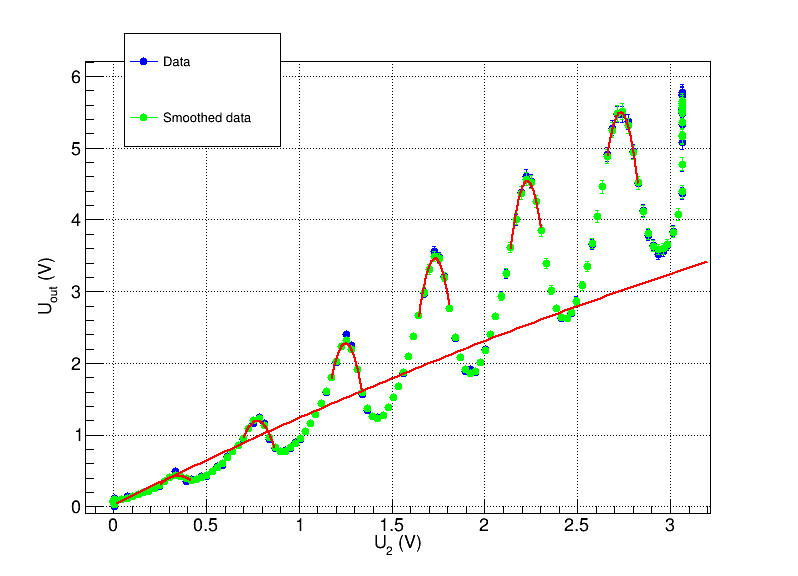
\includegraphics[width=\linewidth]{Hg_4.40_0.94.txt.png}
    \caption{esempio di grafico del Hg ottenuto, ponendo U$_{1}$=4.40V, U$_{3}$=0.94}
    \label{figura1}
\end{figure}
\begin{figure}[h!]
    \centering
    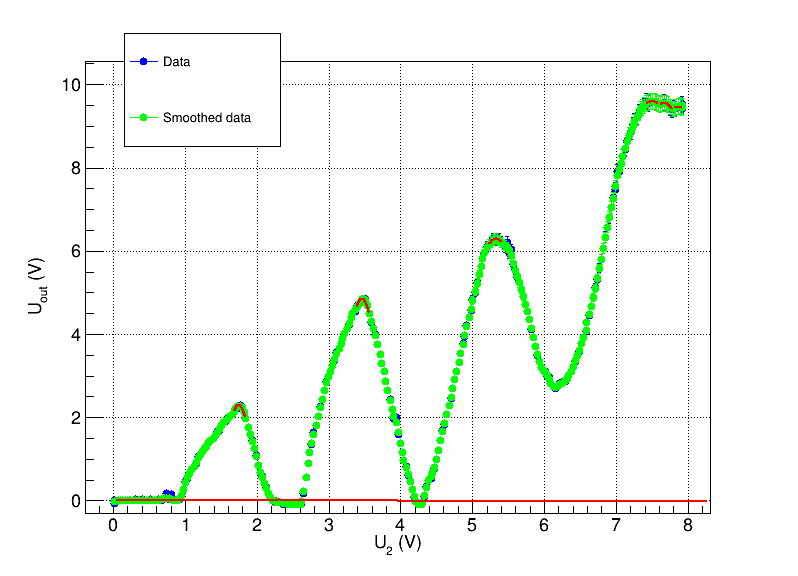
\includegraphics[width=\linewidth]{Ne_1.71_9.01.txt.png}
    \caption{esempio di grafico del Ne ottenuto, ponendo U$_{1}$=1.71V, U$_{3}$=9.01}
    \label{figura1}
\end{figure}





\end{document}
